\chapter{Experimental evaluation} \label{experiments}
I propose to conduct three case studies: a pilot study, a classroom case study, and a public data case study in order to empirically evaluate the capabilities and performance of Software Trajectory framework. The main difference among these experiments lies in the structure of the data used and in the approaches for evaluation. 

My intent behind this studies is to assess the ability of the Trajectory to recognize well known recurrent behavioral patterns (for example Test Driven Development), as well as its ability to discover useful software processes. In addition, these studies will support a classification and extension of the current Hackystat sensor family in order to improve Trajectory's performance. It is quite possible that some of the currently collected sensor data will be excluded from the Trajectory Analysis datasets, while some new ones will be designed and developed in order to capture important features from the studied software development data streams.

The exploratory, evaluative pilot study consists of a set of a small research experiments run on small, custom datasets, and is ongoing with a primary goal to help in the architectural design and development of Trajectory framework. As the secondary goal, these experiments are helping to outline the boundaries of applicability of my approach to certain problems. Section \ref{pilot.evaluation} discusses some of the insights yielded by the pilot study.

The public data case study is based on the use of publicly available Software Configuration Management (SCM) audit trails of the big ongoing software projects such as Eclipse, GNOME etc. Mining of the SCM repositories is a well-developed area of research with much work published \cite{citeulike:5043676}. SCM repositories contain coarse software product artifacts which usually mined with a purpose of discovering various characteristics enlightening software evolution and software process. I am using a mixed approach in this study. In the first phase of this study, I plan to perform SCM audit trail data mining using Trajectory as a tool and following published work as a roadmap in order to discover confirmed patterns in software process artifacts, and thus quantitatively evaluate Trajectory's performance when compared to existing tools. In the second phase, I will develop my own pre-processing and taxonomy mapping of software process artifacts into temporal symbolic series. By using this mapping and Trajectory, I plan to develop a new approach for SCM audit trail mining and possibly discover new evolutionary behaviors within software process. These discovered knowledge will be evaluated through the peer-reviewed publication submitted for the annual MSR challenge \cite{citeulike:5043676}.

The classroom case study is based on the most sophisticated data set. This data will be collected by the Hackystat from Continuous Integration and from individual developers and will contain a fine-grain information about performed software process. The approach I am taking in this study is very similar to the public data case study. I will develop my own taxonomy for mapping of software process artifacts into symbolic temporal data and will apply Trajectory analyses to the low-level software process artifacts in order to discover recurrent behaviors. 

As mentioned, both case studies: public data case study, and classroom case study will involve empirical evaluation. The necessity for this is dictated by the exploratory nature of my research. 

At this point of my research, I can only see that the properties of my approach and it's current implementation in the Software Trajectory framework appear to be very promising. The wealth of developed techniques for temporal symbolic data mining and recent development of the SAX approximation allow to overcome many computational limitations in existing approaches for mining of software process artifacts. Current state of the art implementation of Hackystat provides ability to capture fine-grain software product and process metrics providing previously not-existing richness of data, which, potentially, might reveal new insights. Up to date research in software process discovery indicates the overall feasibility of proposed goals in the discovery of unknown recurrent behaviors in software process. 

Nevertheless, at this early stage of my research, it is impossible to foresee if this new recurrent behaviors will be discovered or assess their meaningfulness or usefulness for real world application. It is possible that this part of research will fail, and I will not be able to discover any novel meaningful knowledge about software process. If so, I will apply every effort to investigate and explain pitfalls of my approach to the software process data mining. Whether it will happen due to the specificity of domain, or due to the insufficiency of the information enclosed in the collected artifacts, or maybe because of inefficiency of augmented methods, through the thorough analyses of failed experiments and collection of the feedback, I will outline boundaries of approach taken in this work and possible future development.

\section{Pilot study}\label{pilot.evaluation}
In order to demonstrate the ability of Trajectory to perform telemetry indexing and temporal recurrent patterns extraction, I have conducted two experiments which provide insights in the use of the motif frequencies and software process event taxonomies. 

\begin{figure}[tbp]
   \centering
   \includegraphics[height=185mm]{cluster_streams.eps}
   \caption{Clustering of telemetry streams for classroom pilot dataset using symbolic approximation and vectors of motif frequencies. While it seems to be meaningful to find correlation between \textit{UnitTest\_Failure} and \textit{CodeIssue} streams unit test, this grouping happened due to the similarity of behavior pattern - short, high amplitude bursts; but note, there is no correlation of features in time .}
   \label{fig:cluster_streams}
\end{figure}

\subsection{Clustering of the Hackystat Telemetry streams}
The main purpose of the this study was to evaluate the ability of PAA and SAX approximations and indexing to capture a temporal specificity of telemetry streams through the discovery of recurrent temporal patterns. Knowing about the frequently misleading results of a time-series clustering \cite{citeulike:227029}, I did not expect to capture much interesting facts, nevertheless the results were encouraging.

The data used in this study was collected from student users of Hackystat during Spring, 2009. This dataset represents Hackystat metrics collected during sixty days of a classroom project by eight students. The following clustering experiments were conducted using the distance between vectors of motif frequencies extracted by indexing of telemetry streams:

\begin{figure}[tbp]
   \centering
   \includegraphics[height=90mm]{dev_clustering.eps}
   \caption{Clustering of developers behavior using symbolic approximation and vectors of motif frequencies. This analysis captured similar development behavior among developers. Developers \#2 and \#7 were consistent (no bursts observed) in both, coding and measuring effort during whole time interval, while all others can be characterized with bursty, inconsistent effort.}
   \label{fig:cluster_developers}
\end{figure}

\begin{itemize}
	\item Clustering of software process related telemetry streams collected from individual developers. I was able to group developers with similar behavioral patterns within clusters, which indicates the feasibility of the classification approach. Figure \ref{fig:cluster_developers} depicts results of this analysis.
	\item Clustering of software product-related telemetry streams by using motif frequencies. I was able to group telemetry streams, but while these groups look intuitively meaningful, the close examination of the stream features suggests that this grouping happened due to the similar temporal behavior on the short stretches. This result, while proving the correctness of approach, indicates it's limitation, pointing that instead of using just motif frequencies, some temporal ordering should be taken into account. Figure \ref{fig:cluster_streams} displays results of this analysis.
\end{itemize}

\subsection{Sequential patterns search}
The second pilot study, focusing on discovery of sequential patterns, was conducted using real data from my own concurrent development of two software projects. While working on the Trajectory framework, I made decision to split the code into two parts: an algorithm implementation library that I named JMotif, and user-interface part called TrajectoryBrowser. While this decision simplified development, it introduced a dependency of TrajectoryBrowser on the JMotif API. As a result of iterative and incremental pattern in my development, I changed the JMotif public API three times, which consequently involved extensive refactoring in the ProjectBrowser code. This dependency can be clearly seen from observing DevTime streams at Figure \ref{fig:sequential_growth} panel $a$. 

\begin{figure}[tbp]
   \centering
   \includegraphics[height=80mm]{sequential_growth.eps}
   \caption{The illustration of finding of sequential $growth \; pattern$ in two DevTime telemetry streams. Panel $a$: The Hackystat ProjectBrowser showing telemetry streams. Panel $b$: the TrajectoryBrowser showing same telemetry streams along with identified pattern. Panel $c$: the symbolic representation of streams with highlighted pattern.}
   \label{fig:sequential_growth}
\end{figure}

In order to capture this dependency pattern in two Telemetry streams, representing the daily amount of development time spent on the TrajectoryBrowser and JMotif projects, I defined a synthetic \textit{growth pattern} as the large positive delta value between previous and current day effort. By transforming Telemetry streams with this simple rule in the symbolic form, I obtained a two dimensional symbolic time series, where letter $G$ represents a growth pattern, see Figure \ref{fig:sequential_growth} panel $c$. I defined a formal rule for \textit{sequential growth} pattern as the pattern like $G_{JMotif}\; \rightarrow \; G_{TrajectoryBrowser}$ where distance between these $G$s is less than three days. By application of this rule I identified a pattern which exactly corresponds to my experience. 

While this experiment was designed with a purpose and does not provide any value in the dependencies discovery, the ``sequential growth'' pattern and past effort information can be used in the estimation of effort needed for requested software changes.
